\section{Periodic Classification}

\begin{multicols}{2}


\section*{The Periodic Table} % Source 122


%\subsection{Classification in Daily Life}
%
%\begin{center}
%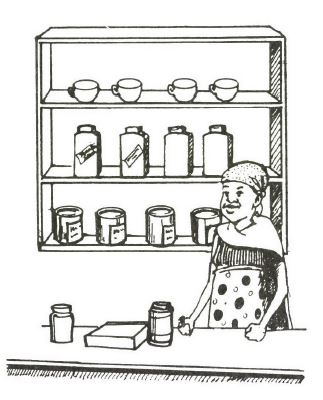
\includegraphics[width=0.35\textwidth]{./img/source/classification.jpg}
%\end{center}
%
%\begin{description*}
%%\item[Subtopic:]{}
%%\item[Materials:]{}
%%\item[Setup:]{}
%\item[Procedure:]{Observe how the goods at the local store are
%arranged on the shelves. }
%%\item[Hazards:]{}
%\item[Questions:]{Can you find a pattern
%in the arrangement on the shelves?}
%\item[Observations:]{The goods
%are probably arranged firstly in large groups i.e.
%food stuffs, non-food stuffs and then again into
%smaller groups such as foods in tins, bags,
%bottles, etc.}
%%\item[Theory:]{}
%%\item[Applications:]{}
%%\item[Notes:]{}
%\end{description*}

\subsection{Arranging Shapes}

\begin{center}
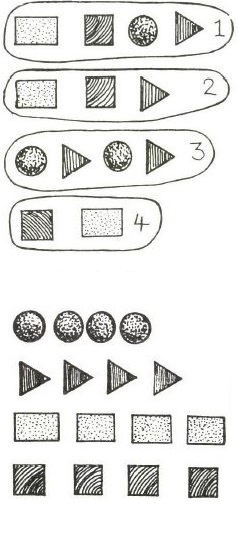
\includegraphics[width=0.4\textwidth]{./img/source/arranging-shapes.jpg}
\end{center}

\begin{description*}
%\item[Subtopic:]{}
\item[Materials:]{Paper/manila or card, scissors, coloured pencils or markers}
%\item[Setup:]{}
\item[Procedure:]{Make several of each of the following
shapes: squares (3 $\times$ 3 cm), triangles (3 cm sides),
rectangles (3 $\times$ 4 cm), circles (3 cm diameter). Make some of the same shape which are smaller and larger than these as well. Colour them all differently (not according to shape).
Mix the shapes and then sort them according to
a chosen feature. }
%\item[Hazards:]{}
\item[Questions:]{How many different ways can
you find of grouping the shapes?}
%\item[Observations:]{}
%\item[Theory:]{}
%\item[Applications:]{}
%\item[Notes:]{}
\end{description*}

\vfill
\columnbreak

\subsection{Bottle Cap Periodic Table}

\begin{center}
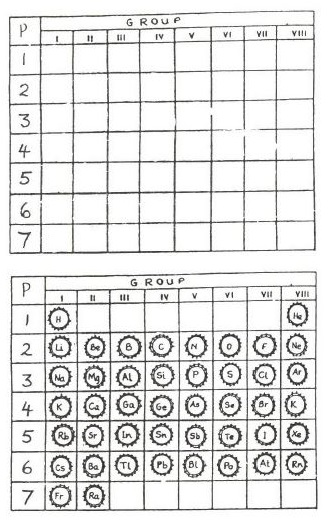
\includegraphics[width=0.49\textwidth]{./img/source/periodic-table.jpg}
\end{center}

\begin{description*}
%\item[Subtopic:]{}
\item[Materials:]{Chalk/manila paper, markers, bottle caps, seeds (optional)}
\item[Setup:]{Ask the students to draw an empty chart
of the periodic table. Then let them write the names of the
elements inside the bottle caps.
Use different colours for metals, semi-metals
and non-metals. Bottle caps for all elements are
needed.}
\item[Procedure:]{Ask the pupils
to place the appropriately labeled bottle caps on
the correct squares. As an extension, put seeds around
the bottle tops to represent the valence electrons.}
%\item[Hazards:]{}
%\item[Questions:]{}
%\item[Observations:]{}
%\item[Theory:]{}
%\item[Applications:]{}
%\item[Notes:]{}
\end{description*}

\vfill
\columnbreak

\subsection{Periodic Table Game}

\begin{center}
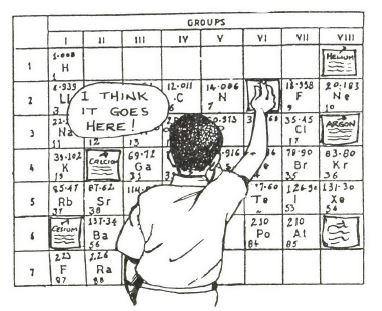
\includegraphics[width=0.49\textwidth]{./img/source/periodic-table-game.jpg}
\end{center}

\begin{description*}
%\item[Subtopic:]{}
\item[Materials:]{Manila/flipchart paper, markers, cards, tape}
\item[Setup:]{Create a permanent periodic table on manila or flipchart paper to post in the classroom. Make a series of cards for elements as
shown above so they fit into the spaces of your
periodic table. }
\item[Procedure:]{Hang or place cards around the classroom and have students each choose one, read it aloud and place it onto the
appropriate position of the table. The
student should be asked to explain his/her
answer. This exercise also helps to develop
language skills (speaking and reading).}
%\item[Hazards:]{}
%\item[Questions:]{}
%\item[Observations:]{}
%\item[Theory:]{}
%\item[Applications:]{}
\item[Notes:]{You can also give each student one or two elements to make on the cards and then bring them together for the class to share.}
\end{description*}

\vfill
\columnbreak

\subsection{Periodic Table Guess Who?}

\begin{center}
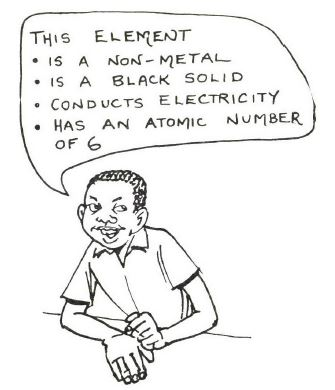
\includegraphics[width=0.45\textwidth]{./img/source/periodic-guess-who.jpg}
\end{center}

\begin{description*}
%\item[Subtopic:]{}
\item[Materials:]{Paper, beans/seeds/etc.}
%\item[Setup:]{}
\item[Procedure:]{A game for 2 players. Each student thinks of an element from the periodic table. Students take turns asking `yes' or `no' questions to determine which element the other is thinking of. For example, ``Is your element a noble gas?'' or ``Does your element have 3 energy levels?'' The first player to guess the other player's element is the winner.}
%\item[Hazards:]{}
%\item[Questions:]{}
%\item[Observations:]{}
%\item[Theory:]{}
%\item[Applications:]{}
\item[Notes:]{Have students draw a periodic table and use markers (beans, corn kernels, etc.) to cover elements which they have eliminated from their questions.}
\end{description*}

%==================================================================================================%


\end{multicols}

\begin{center}
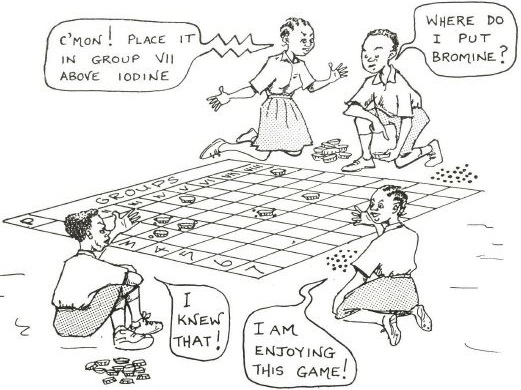
\includegraphics[width=0.7\textwidth]{./img/source/periodic-students.jpg}
\end{center}


\pagebreak